
In some cases the assumption can be made that the object we wish to sudy has an 
axisymmetric geometry, for example a plume:

\begin{center}
a)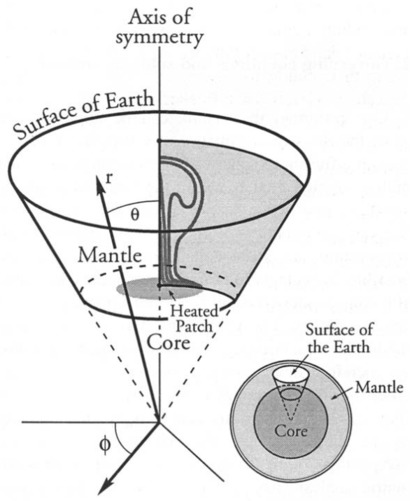
\includegraphics[width=5cm]{images/axisymmetry/keki97}
b)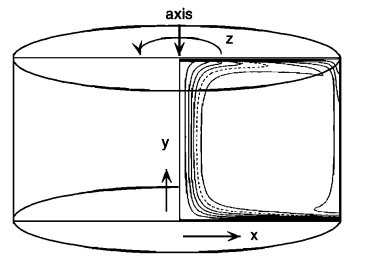
\includegraphics[width=5cm]{images/axisymmetry/lesy96a}
c)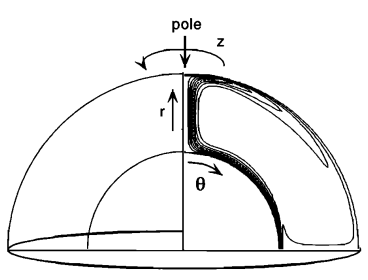
\includegraphics[width=5cm]{images/axisymmetry/lesy96b}\\
{\captionfont a)Taken from Kellogg \& King (1997) \cite{keki97}.
b,c) Taken from Leitch \etal (1996) \cite{lesy96}.}
\end{center}

Looking at the figure above we see that there are in fact two cases: axisymmetry in 
cylindrical coordinates (b) and axisymmetry in spherical coordinates (c).

%---------------------------------------
\subsubsection{In cylindrical coordinates}

The velocity vector is $\vec{\upnu}=(\upnu_r,\upnu_\theta,\upnu_z)$. 
Due to the symmetry we have $\upnu_\theta=0$, $\partial_\theta \rightarrow 0$ 
and the Stokes equations 
then become \footnote{\url{https://en.wikipedia.org/wiki/Navier-Stokes_equations}}

\begin{eqnarray}
-\frac{\partial p}{\partial r} + \eta
\left(
\frac1r \frac{\partial}{\partial r} ( r  \frac{\partial \upnu_r}{\partial r}   ) 
+  \frac{\partial^2 \upnu_z}{\partial z^2} - \frac{\upnu_r}{r^2}
\right) +\rho g_r&=& 0 \\
-\frac{\partial p}{\partial z} + \eta
\left(
\frac1r \frac{\partial}{\partial r} ( r  \frac{\partial \upnu_r}{\partial r}   ) 
+  \frac{\partial^2 \upnu_z}{\partial z^2} 
\right) +\rho g_r&=& 0 \\
\frac1r \frac{\partial}{\partial r} (r \upnu_r) + \frac{\partial \upnu_z}{\partial z} &=& 0
\end{eqnarray}




%---------------------------------------
\subsubsection{In spherical coordinates}


THESE EQUATIONS SHOULD BE CHECKED and RE-CHECKED !!

Assuming the flow velocity does not depend on $\phi$ ($\partial_\phi =0$) and therefore also that $\upnu_\phi=0$
\[
0=-\frac{\partial p}{\partial r} + f_r + \eta \left(\Delta v_r - \frac{2v_r}{r^2} -\frac{2}{r^2} \frac{\partial v_\theta}{\partial \theta} - \frac{2 v_\theta \cot \theta }{r^2} \right)
\]
\[
0 = -\frac{1}{r} \frac{\partial p}{\partial \theta} + \eta \left(\Delta v_\theta + \frac{2}{r^2} \frac{\partial v_r}{\partial \theta}  - \frac{v_\theta}{r^2 \sin^2 \theta} \right)
\]
with
\[
\Delta = \frac{1}{r^2} \frac{\partial }{\partial r}\left( r^2 \frac{\partial }{\partial r}\right)
+\frac{1}{r^2 \sin\theta} \frac{\partial }{\partial \theta}
\left(
\sin\theta \frac{\partial }{\partial\theta}
\right)
\]


\[
\Delta = \frac{1}{r^2} \frac{\partial }{\partial r}\left( r^2 \frac{\partial }{\partial r}\right)
+\frac{1}{r^2 \sin\theta} \frac{\partial }{\partial \theta}
\left(
\sin\theta \frac{\partial }{\partial\theta}
\right)
+ \frac{1}{r^2 \sin^2\theta} \frac{\partial^2 }{\partial\phi^2}
\]

THESE EQUATIONS SHOULD BE CHECKED and RE-CHECKED !!



From \cite{zebi93}:
\begin{equation}
\frac{1}{r^2} \frac{\partial}{\partial r} (r^2 \upnu_r) + 
\frac{1}{r \sin \theta} \frac{\partial}{\partial \theta} (\upnu_\theta \sin \theta)+
\frac{1}{r \sin \theta} \frac{\partial \upnu_\phi}{\partial \phi} = 0
\end{equation}
Pb with 1/r2 ??

\begin{eqnarray}
0 &=& -\frac{\partial p}{\partial r} + (1-\zeta) Ra \; r \; T + 
\frac{1}{r^2}\frac{\partial}{\partial r} \left( 2 \eta r^2 \frac{\partial \upnu_r}{\partial r} \right)
+ \frac{1}{r^2 \sin\theta} \frac{\partial}{\partial\theta} 
\left( \eta \sin\theta \frac{\partial \upnu_r}{\partial\theta} \right)
+\frac{\partial}{\partial \theta} \left(\eta \frac{\partial}{\partial r} \frac{\upnu_\theta}{r} \right)
\end{eqnarray}
where $\zeta=R_i/R_o$


The dimensional form of the energy equation in a spherical axisymmetric geometry is given by
(assuming the conductivity $k$ to be constant):
\[
\rho C_p \left( \frac{\partial T}{\partial t}  + 
\upnu_r \frac{\partial T}{\partial r} + \frac{\upnu_\theta}{r} \frac{\partial T}{\partial \theta}
\right)
=
k \frac{1}{r^2} \frac{\partial}{\partial r} \left( r^2 \frac{\partial T}{\partial r} \right)
+
k \frac{1}{r^2 \sin\theta} 
\frac{\partial}{\partial \theta} \left( \sin\theta \frac{\partial T}{\partial \theta}  \right) 
...
\]

THESE EQUATIONS SHOULD BE CHECKED and RE-CHECKED !!



